\chapter{Special Topic: The Higgs Boson}\label{ap:spec_higgs}

\index{Higgs!boson}
This chapter summarizes the importance of the Higgs boson in QFT and outlines
experiments leading up to the discovery of the Higgs boson.
First we discuss the issues of boson and fermion masses and explain
how the Higgs mechanism allows for such particles to exist in gauge invariant
theories. We apply this method to the standard model, and from this deduce
properties of the Higgs boson. The paper finally turns to preliminary results 
from LEP and Tevatron before concluding with the 2012 discovery at the LHC.

The Higgs mechanism is an example of SSB, so if you like, you can refresh
yourself by looking to \secref{sec:ssb}. In this chapter we will
also pay attention to the location of Lorentz indices again, as we
work with the physical Minkowski metric.

Since this chapter was adapted from a project I did as a grad student in 2014,
this chapter is likely not current.

\section{Gauge invariance in QFT}

Building a gauge invariant Lagrangian is at the heart of constructing theories
of modern particle physics. There are a couple of reasons for demanding that a
theory not depend on gauge. For one, gauge invariant theories have the nice
property of being renormalizable, a fact shown in 1972 by t'Hooft and Veltman 
\cite{t_hooft_regularization_1972}. Perhaps more importantly, utilizing gauge
invariance is an elegant way of deriving Lagrangians complete with terms
describing the observed interactions between gauge bosons and matter fields.

For example, consider a Lagrangian of the form
\begin{equation}
  \label{eq:genLagr}
  \Lagr=\bar{\psi}\slashed{D}\psi-\frac{1}{4}\tr F_{\mu\nu}F^{\mu\nu} ,
\end{equation}
where $D_{\mu}$ and $F_{\mu\nu}$ are respectively the gauge covariant
derivative and field strength
This is invariant under local gauge transformations. 
As mentioned previously, this is a desirable feature for the
Lagrangian to have, and hence it is a solid foundation off of which to build
a theory.

One notable feature about the Lagrangian~\eqref{eq:genLagr} is that
it doesn't allow for particles corresponding to gauge fields to have masses.
Consider for instance a naive mass term of the form $mA^{\mu}A_{\mu}$. Then 
under a local gauge transformation we would have
\begin{equation}
  \begin{aligned}
  mA'^{\mu}A'_{\mu}&=mUA_{\mu}U^{\dagger}UA^{\mu}U^{\dagger} \\
                   &=mUA_{\mu}A^{\mu}U^{\dagger},
  \end{aligned}
\end{equation}
which is in general not invariant. This suggests that the gauge bosons are
massless. While this is no contradiction for QED or QCD, this is in direct
opposition of observation that weak vector bosons have mass. Furthermore
electron mass terms of the form $\bar{\psi}_{L}\psi_{R}+
\bar{\psi}_{R}\psi_{L}$ are not invariant under 
$\SU(2)_{L}\times \U(1)_{Y}$ gauge transformations since left- and 
right-handed fermions
transform differently \cite{dittmaier_higgs_2013}.

\section{The Higgs mechanism}

\index{Higgs!mechanism}
Let us examine the mechanism responsible for reconciling the observation of 
massive gauge bosons with the desire for our theory to be gauge invariant. For 
the sake of simplicity, we consider a complex scalar field under a $\U(1)$ 
symmetry (scalar electrodynamics), but this procedure generalizes to 
non-abelian theories \cite{srednicki_quantum_2007}. 
We specify our Lagrangian by 
\begin{equation}
  \label{eq:HLagr1}
  \Lagr=-(D_{\mu}\phi)^{\dagger}D^{\mu}\phi-V(\phi)
              -\frac{1}{4}F_{\mu\nu}F^{\mu\nu},
\end{equation}
where $\phi$ is a complex scalar field, and
\begin{equation}
  \label{eq:pot}
  V(\phi)=m^{2}\phi^{\dagger}\phi+\frac{1}{4}\lambda(\phi^{\dagger}\phi)^{2}.
\end{equation}
We can identify the first term in \equatref{eq:pot} as representing the mass of
the particle and the second as representing self interactions of the field.
In the case $m^2>0$, the potential has a minimum at $|\phi|=0$, and we obtain 
the scalar electrodynamics to which we are accustomed. Now let us allow 
$m^2<0$. In this case, $V(\phi)$ takes its minimum on the circle defined by
\begin{equation}
  \label{eq:v2}
  \Re[\phi]^2+\Im[\phi]^2=v^2\equiv\frac{-4m^2}{\lambda}.
\end{equation}
The physical vacuum state will correspond to a point on this circle. (This
is the same case as depicted in Fig.~\ref{fig:ssb}.) Choosing a state 
from among this continuum thus breaks the original
$\U(1)$ symmetry of the Lagrangian, which is an example of SSB. 

The vacuum expectation value (VEV) of the field is
\begin{equation}
  \bra{0}\phi(x)\ket{0}=\frac{v}{\sqrt{2}}.
\end{equation}
Let us find excited states by carrying out a perturbative expansion of $\phi$ 
about the vacuum state. We write
\begin{equation}
  \label{eq:phixpand}
  \begin{aligned}
  \phi(x)&=\frac{1}{\sqrt{2}}\big(v+h(x)+i\chi(x)\big) \\
         &\approx\frac{1}{\sqrt{2}}\big(v+h(x)\big)
                  e^{i\chi(x)/v}
  \end{aligned}
\end{equation}
to first order in the fields. (Here $h$ and $\chi$ are real.) Plugging 
\equatref{eq:phixpand} into \eqref{eq:pot}, using the definition of 
$v^2$, and throwing away the constant term (which of course doesn't change the 
physics) yields
\begin{equation}
  \label{eq:potnew}
  V(\phi)=\frac{1}{4}\lambda v^{2}h^{2}+\frac{1}{4}\lambda vh^{3}
          +\frac{1}{16}\lambda h^{4}.
\end{equation}
Since $V(\phi)$ is independent of $\chi$, the field must be massless,
and $\chi$ is the Goldstone boson for the broken symmetry. Since the
Lagrangian is gauge invariant, we can eliminate $\chi$ by making the
local transformation
\begin{equation}
  \phi(x)\to\phi'(x)=e^{-i\chi(x)/v}\phi(x).
\end{equation}
This choice of gauge is called the {\it unitary gauge}\index{unitary gauge}. 
In the unitary gauge
$\phi(x)$ becomes
\begin{equation}
  \label{eq:phinew}
  \phi(x)=\frac{1}{\sqrt{2}}\big(v+h(x)\big).
\end{equation}
We are finally in a position to physically interpret the fields. Plugging 
\equatref{eq:phinew} and \eqref{eq:potnew} into the first term of 
\eqref{eq:HLagr1} gives
\begin{equation}
  \label{eq:kin}
  \begin{aligned}
    -(D_{\mu})^{\dagger}(D^{\mu})&=-\frac{1}{2}(\partial_{\mu}h+ig(v+h)A_{\mu})
                                (\partial^{\mu}h-ig(v+h)A^{\mu}) \\
         &=-\frac{1}{2}\partial_{\mu}h\partial^{\mu}h 
           -\frac{1}{2}g^{2}(v^{2}+h^{2}+2vh)A_{\mu}A^{\mu}. 
  \end{aligned}
\end{equation} 
Viewed in this way, the gauge field has a mass
\begin{equation}
  M_{A}=gv.
\end{equation}
This process of eliminating the dependence of the Lagrangian on the Goldstone
boson combined while the gauge boson acquires a mass is called the {\it Higgs
mechanism}\index{Higgs!mechanism}. Furthermore the term quadratic in 
$h^2$ in \equatref{eq:potnew} shows the mass of the {\it Higgs field} 
$h$\index{Higgs!field} is
\begin{equation}
  M_{h}=\sqrt{2\lambda}v.
\end{equation}

Thus we see that out of our original Lagrangian falls a mass for the gauge
\index{Higgs!boson}
boson as well as for the {\it Higgs boson}, the boson corresponding to the
Higgs field. The Higgs mechanism has an admirable neatness to it. After all,
we found the boson by simply allowing $m^2<0$, which is perfectly justifiable
since we don't know {\it a priori} whether $\phi$ corresponds to a physical 
mass; in fact the Higgs mechanism suggests that rather than $\phi$, the
fields $h$ and $A^{\mu}$ are physical. Astonishingly, the Higgs mechanism
can also be used to fix the electron mass problem, which we will see in the
next section.

\section{The Standard Model Higgs}
The full Lagrangian of the Standard Model in its most general form is
\begin{equation}
  \label{eq:LSM}
  \Lagr_{\rm SM}=\Lagr_{\rm YM}+\Lagr_{\rm ferm}+\Lagr_{\rm Higgs}
                               +\Lagr_{\rm Yuk},
\end{equation}
where
\begin{equation}
  \label{eq:Ldefs}
  \begin{aligned}
    \Lagr_{\rm YM}&=-\frac{1}{4}W_{\mu\nu}^iW^{\mu\nu,i}
                -\frac{1}{4}B_{\mu\nu}B^{\mu\nu}
                -\frac{1}{4}G_{\mu\nu}^aG^{\mu\nu,a}, \\
    \Lagr_{\rm ferm}&= i\bar{\Psi}_{L}\slashed{D}\Psi_{L}
                  +i\bar{\psi}_{\ell_R}\slashed{D}\psi_{\ell_R}
                  +i\bar{\Psi}_{Q}\slashed{D}\Psi_{Q}
                  +i\bar{\psi}_{u_R}\slashed{D}\psi_{u_R}
                  +i\bar{\psi}_{d_R}\slashed{D}\psi_{d_R}, \\
    \Lagr_{\rm Higgs}&=(D_{\mu}\Phi)^{\dagger}(D^{\mu}\Phi)-V(\Phi), \\
    \Lagr_{\rm Yuk}&=-\bar{\Psi}_{L}G_{\ell}\psi_{\ell_R}\Phi
                 -\bar{\Psi}_{Q}G_{u}\psi_{u_R}\widetilde{\Phi}
                 -\bar{\Psi}_{Q}G_{d}\psi_{d_R}\Phi+h.c.,
  \end{aligned}
\end{equation}
$i$ runs from 1 to 3, and $a$ runs from 1 to 8. \cite{dittmaier_higgs_2013}. 
The interpretation 
of the first two terms is straightforward: The field strength 
tensors in the Yang-Mills part $\Lagr_{\rm YM}$ contain the 
kinetic terms of gauge 
fields as well as their self-interactions; $W$, $B$, and $G$ correspond to the 
weak, electromagnetic, and strong interactions, respectively. Meanwhile the 
fermion term $\Lagr_{\rm ferm}$ includes the couplings of gauge fields to the 
fermions, which are contained in
\begin{equation}
  D_{\mu}\equiv\partial_{\mu}+igI_{W}^{i}W_{\mu}^{i}
                  +ig'\frac{Y}{2}B_{\mu}+ig''T_{c}^{a}G_{\mu}^{a}.
\end{equation}
Here $I_{W}^{j}$, $Y_{W}$, and $T_c^{a}$ are the generators of the respective 
gauge groups, expressed in the same representation as the fermions on which 
they act.

To interpret the $\Lagr_{\rm Higgs}$, we employ the Higgs mechanism 
as before. The potential is
\begin{equation}
  \label{eq:Higgpot}
  V(\Phi)=m^2(\Phi^{\dagger}\Phi)+\frac{\lambda}{4}(\Phi^{\dagger}\Phi)^2
\end{equation}
and $\Phi$ is a complex scalar doublet
\begin{equation}
  \label{eq:newphi}
  \Phi=
  \begin{pmatrix}
    \phi^{+} \\
    \phi^{0}
  \end{pmatrix},
\end{equation}
where $\phi^{+}$ has charge $+e$ and $\phi^{0}$ has zero charge. We minimize
\equatref{eq:Higgpot} and spontaneously break the $\SU(2)_{L}\times\U(1)_{Y}$ 
symmetry while requiring the minimum correspond to a VEV only of $\phi^{0}$.
After expanding about the vacuum state in the unitary 
gauge (thereby eliminating any Goldstone bosons) we can write
\begin{equation}
  \label{eq:Higgsphi}
  \Phi=\frac{1}{\sqrt{2}}
  \begin{pmatrix}
    0 \\
    v+h
  \end{pmatrix}.
\end{equation}
To find the form of $\Lagr_{\rm Higgs}$ in this gauge, we plug in 
\equatref{eq:Higgsphi}
as well as the definitions of $W^{\pm}_{\mu}$ and the {\it weak mixing angle} 
$\theta_W$,
\begin{equation}
  W^{\pm}_{\mu}\equiv\frac{1}{\sqrt{2}}(W^{1}_{\mu}\mp iW^{2}_{\mu}),
  \ \ c_W\equiv\cos(\theta_W)\equiv\frac{gg'}{g^2+(g')^2},
\end{equation}
to obtain
\begin{equation}
  \label{eq:LagrHiggs}
  \begin{aligned}
    \Lagr_{\rm Higgs}&=\frac{1}{2}\partial_{\mu}h\partial^{\mu}h
                   +\frac{g^4}{4}(v+h)^{2}W^+_{\mu}W^{-\mu} \\
       & ~~~~~     +\frac{g^2}{8c_{W}^{2}}(v+h)^{2}Z_{\mu}Z^{\mu}
                   +\Big(\frac{\mu^2}{2}-\frac{\lambda}{16}\Big)(v+h)^{2} \\
       &=\frac{1}{2}\partial_{\mu}h\partial^{\mu}h
         -\frac{1}{2}M_{h}^{2}h^2 + M_{W}^{2}W^+_{\mu}W^{-\mu} \\
       & ~~~~~ +\frac{1}{2}M_{Z}^{2}Z_{\mu}Z^{\mu} 
         + gM_{W}hW^+_{\mu}W^{-\mu}
         +\frac{g^2}{4}h^{2}W^+_{\mu}W^{-\mu} \\
       & ~~~~~ +\frac{gM_{Z}}{2c_{W}}hZ_{\mu}Z^{\mu}
         +\frac{g^2}{4c_{W}^{2}}h^{2}Z_{\mu}Z^{\mu}
         -\frac{gM_{h}^2}{4M_W}h^3 - \frac{g^{2}M_{h}^2}{32M_{W}^2}h^4,
  \end{aligned}
\end{equation}
where we have neglected a constant term (as before) and used
\begin{equation}
  M_W\equiv\frac{gv}{2},\ \ M_Z\equiv\frac{M_W}{c_W},\ \
  M_h\equiv\sqrt{2m^2},\ \ v\equiv 2\sqrt{\frac{m^2}{\lambda}}.
\end{equation}
Hence we see that through SSB, the Higgs field has 
lent mass terms to the previously massless weak vector bosons, and that the 
photon has remained massless as desired. Perhaps more to the point of this 
section, we are able to glean important phenomenological predictions about the 
Higgs boson from the form of \equatref{eq:LagrHiggs}. Namely,
\begin{enumerate}
  \item the term quadratic in $h$ shows the Higgs has a mass $M_h$;
  \item the Higgs is spin-0 because the Higgs field is a scalar;
  \item it is neutral, since it is a perturbation of the vacuum state,
        which we required to be neutral when we broke the 
        $\SU(2)_{L}\times\U(1)_{Y}$ symmetry;
  \item it is CP even since, again, it is a vacuum excitation, and thus 
        carries the same quantum numbers as the vacuum;
  \item the three-vertex coupling of the Higgs to the $V=W,$ $Z$ bosons 
        is proportional to the mass of those bosons $M_V$, which we see from 
        $hV^{\dagger}V$ terms, while the four-vertex coupling is proportional
        to $M_{V}^2$, which comes from $h^{2}V^{\dagger}V$ terms (more
        precisely the coupling of the $hV^{\dagger}V$ term is $gM_{V}$, so we
        can also think of the coupling as being proportional to $M_{V}^{2}/v$,
        and similarly of the $h^{2}V^{\dagger}V$ coupling as proportional
        to $M_{V}^{2}/v^{2}$); 
        \vspace{9mm}
  \item the last two terms show cubic and quartic Higgs self-interactions;
  \item and the $W$ boson mass, $Z$ boson mass, and weak mixing angle are 
        related by $$\cos(\theta_W)=\frac{m_W}{m_Z}.$$
\end{enumerate}

Finally we consider the Yukawa part of the Standard Model Lagrangian. The
$h.c.$ in $\Lagr_{\rm Yuk}$ includes the hermitian conjugates of all the terms
preceding it. $\ell$, $u$, and $d$ refer to charged leptons, up-type quarks
(up, charm, top), and down-type quarks (down, strange, bottom), respectively.
$\widetilde{\Phi}$ is the Higgs doublet with opposite quantum numbers as
$\Phi$ and conjugated charge. The matrices $G_f$ mix left- and right-handed 
parts of different generations of the fermion type $f$ 
\cite{dittmaier_higgs_2013}. 

We can remove this mixing by transforming these matrices from the current 
{\it flavor basis} to the basis in which they are diagonal, the {\it mass 
basis}. In this basis
\begin{equation}
  G_f=\frac{\sqrt{2}}{v}\diag(m_{f_1},m_{f_2},m_{f_3}), 
\end{equation}
and $m_{f_i}$ can be interpreted as the mass of fermion $f_i$. Substituting
\equatref{eq:newphi} into $\Lagr_{\rm Yuk}$ and transforming to the 
unitary gauge, the Yukawa term becomes
\begin{equation}
  \Lagr_{\rm Yuk}=-\sum\limits_{f}m_{f}\Big(1+\frac{H}{v}\Big)
            (\bar{\psi}_{L_f}\psi_{R_f}+\bar{\psi}_{R_f}\psi_{L_f}),
\end{equation} 
where the sum is over all fermion flavors and all generations 
\cite{dittmaier_higgs_2013}. Cast
in this form, the Yukawa term gives us the prediction that
\begin{enumerate}
  \setcounter{enumi}{7}
  \item the Higgs boson couples to each fermion $f$ with strength $y_f=m_f/v$.
        This coupling constant is known as the {\it Yukawa coupling}.
\end{enumerate}
Hence we see that the issue of fermion masses has also been solved by the
Higgs mechanism. We note that in the lepton sector, the
change of basis is furnished by the same matrices for neutrinos as it is for
their corresponding charged particles only in the limit of massless neutrinos
\cite{dittmaier_higgs_2013}.


\section{How to find the Higgs}
Armed with our predictions from the previous section, we are in a favorable
position to motivate searches for the Higgs boson. We will see how searches for
the Higgs helped place a tight window on its expected mass, even though the 
mass is, in principle, a free parameter.
\begin{figure}
  \centering
  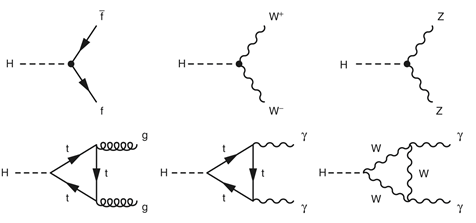
\includegraphics[width=0.75\textwidth,height=0.75\textheight,keepaspectratio]
                {pictures/higgs_decays.png}
  \caption{Example decay modes of the Higgs boson. Image taken from Thomson
           Figs. 17.14 and 17.16  \cite{thomson_modern_2013}.}
  \label{fig:exhiggsdecays}
\end{figure}

A preliminary step in accomplishing this goal is to decide which search 
channels to use. Knowing that the coupling of the Higgs boson to elementary 
bosons and fermions increases with the masses of those particles, one might be 
tempted to pick search channels whose Feynman diagrams involve the most massive
particles that are kinematically allowable. However there are 
also practical theoretical and experimental constraints that might make a 
channel with a smaller branching ratio a better candidate for search. The 
means to trigger signal events with high efficiency, suppress background 
radiation (e.g. multi-jet final states from other QCD interactions during a
hadron-hadron collision), and estimate uncertainties in signal and background 
predictions are also highly important, and were therefore taken into account by
scientists investigating the Higgs.

In addition to production channels, experimenters must decide which
decay modes to look for. Looking at the vertex factors above, the Higgs 
can decay into fermion-antifermion pairs as well as $W^{+}W^{-}$ and $ZZ$.
Furthermore the Higgs can decay into gluon-gluon and photon-photon pairs
through virtual quark and weak vector boson loops. For example Higgs decay
Feynman diagrams, see Fig.~\ref{fig:exhiggsdecays},

As detailed in Dittmaier and Schumacher \cite{dittmaier_higgs_2013}, 
there were no tight
constraints on the Higgs mass prior to investigations at the Large Electron
Positron Collider (LEP). The primary search
channel there was $ZH$ production via ``Higgs-strahlung", for which the diagram
is shown in Fig.~\ref{fig:higgsstrahlung}. 
The signal used at LEP was based on the $H\to b\bar{b}$ 
decay, which is not surprising since the bottom quark is the most 
massive fermion in the decay $H\to f\bar{f}$ for which $M_{h}>2M_{f}$. During
the LEP1 era (1989-1995), the collider operated at a CM energy of about $M_Z$. 
By the end of this era, the internal experiments ALEPH, DELPHI, L3, and OPAL 
together excluded Higgs boson masses below 63.2 GeV. Next the CM energy was
increased periodically from ~130 GeV in 1995 to 200 GeV in 2000--this is the
LEP2 era. By this time, the ability to identify b-flavored jets had been
greatly improved, which made it easier to distinguish signal and background. 
The final results of LEP2 showed a promising indication of the existence of
the Higgs, but were not strong enough to claim a discovery. Ultimately
the LEP2 experiments were able to exclude Higgs masses below 115 GeV with at
least 95\% confidence.

\begin{figure}
  \centering
  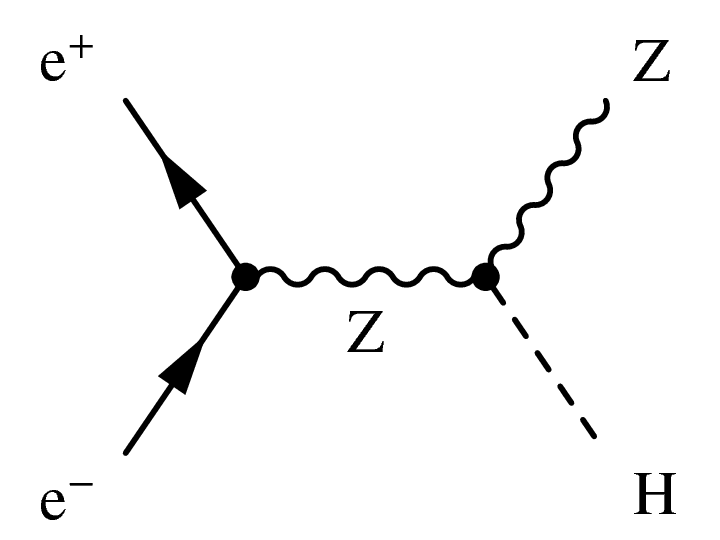
\includegraphics[width=0.40\textwidth,height=0.40\textheight,keepaspectratio]
                {pictures/higgsstrahlung.png}
  \caption{Leading order diagram for the production channel Higgs-strahlung. 
           Image taken from Simon \cite{simon_prospects_2013}.}
  \label{fig:higgsstrahlung}
\end{figure}

Besides electron-positron colliders, Higgs searches and exclusion experiments
have also taken place at hadron colliders, most notably the Tevatron at
Fermilab and the LHC at CERN. In 2001 the Tevatron Run II started with a CM 
energy of ~2 TeV. Running until 2011, the precision measurements at the
Tevatron suggested that the Higgs mass is less than 150 GeV, and not likely
larger than 200 GeV \cite{thomson_modern_2013}.

\section{Experimental evidence for the Higgs}
Between results from the LEP collider and Tevatron, high energy physicists
could have expected the Higgs mass to lie between 115 and 150 GeV. Nevertheless
the LHC and its two experiments ATLAS and CMS were designed to explore the
entire mass range from 115 GeV to ~1 TeV, which is the largest the Higgs mass
can be without violating unitarity \cite{dittmaier_higgs_2013}. The LHC is currently
the highest energy particle collider ever built and the highest luminosity 
proton-proton collider. Starting in 2010, the LHC operated at a CM energy of 7+
TeV, a drastic improvement over the energies of previous particle accelerators.
\begin{figure}
  \centering
  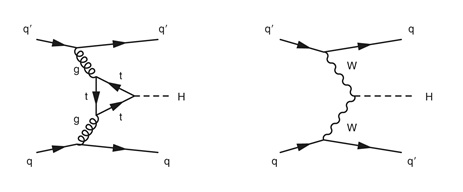
\includegraphics[width=0.75\textwidth,height=0.75\textheight,keepaspectratio]
                {pictures/higgs_prod_hadrons.png}
  \caption{Leading order diagrams for the Higgs boson production channels
           (left) gluon fusion and (right) vector boson fusion. Image taken 
           from Thomson Fig. 17.17 \cite{thomson_modern_2013}.}
  \label{fig:higgsfusion} 
\end{figure}

The primary search channels at the LHC were gluon fusion and vector boson
fusion, the Feynman diagrams of which are shown in Fig.~\ref{fig:higgsfusion}. 
Because of the 
heavy masses of the top quarks, the gluon fusion process has a large cross 
section. However the gluon fusion process also leads to QCD radiation, which 
can make final states of this production channel difficult to distinguish from 
background QCD interactions. Meanwhile, the vector boson fusion final states 
consist only of Higgs boson decay products and forward jets from the colliding 
protons, making them more easily identifiable. Similarly the most
sensitive decay modes investigated were $H\to\gamma\gamma$, $H\to ZZ^{*}\to
\ell_{1}^{+}\ell_{1}^{-}\ell_{2}^{+}\ell_{2}^{-}$ (where $\ell_i$ is an 
electron or muon and the asterisk indicates that the $Z$-boson is off 
shell), and
$H\to WW^{*}\to e\nu_{e}\mu\nu_{\mu}$ because they can be more easily
distinguished from the background. The decays $H\to\gamma\gamma$ 
and $H\to ZZ^{*}\to4\ell$ also have the advantage that the mass of the Higgs 
can be more easily reconstructed from the masses of their decay products
\cite{dittmaier_higgs_2013}.

Although ATLAS and CMS searched the final states $\gamma\gamma$, $ZZ^{*}$,
$WW^{*}$, $\tau^{+}\tau^{-}$, and $b\bar{b}$, the most significant data came
from the $H\to \gamma\gamma$ and $H\to\ ZZ^{*}\to4\ell$ modes \cite{thomson_modern_2013}.
The reconstructed invariant mass distributions from ATLAS and CMS provided
statistically credible evidence for the existence of a new particle. Two
of the most significant distributions are shown in 
Fig.~\ref{fig:higgsevidence}. In the ATLAS plot,
each event is weighted with the probability that it is kinematically compatible
with Higgs production and decay \cite{thomson_modern_2013}. We can see in both plots more events
than is expected from the background around a mass of 125 GeV, which we
identify as the Higgs. The peak at 91 GeV in the CMS plot can be attributed
to $Z$-boson production \cite{thomson_modern_2013}. 

Ultimately the discovered particle masses for each experiment were determined 
\cite{dittmaier_higgs_2013} to be
\begin{equation}
  \begin{aligned}
  M_{h({\rm ATLAS})}&=126.0\pm0.4(\text{stat})
                \pm0.4(\text{sys})\ \text{GeV}, \\
  M_{h({\rm CMS})}&=125.3\pm0.4(\text{stat})\pm0.5(\text{sys})\ \text{GeV}.
  \end{aligned}
\end{equation}
The fact that the new particle decays into a pair of particles with the same
spin and zero net charge shows that it is electrically neutral and has
integer spin. Hence by the spin statistics theorem, it is a neutral boson.
Furthermore by the Landau-Yang theorem, the fact that it can decay into two 
identical, massless, spin-1 particles shows that it cannot be a spin-1 particle
itself. Moreover the CMS Collaboration has recently been able to exclude many
spin-2 models for the Higgs at a confidence level of 99\% or higher 
\cite{khachatryan_constraints_2015}.
These observations together suggest that the particle found at the LHC is 
almost certainly the Higgs boson.

\begin{figure}
  \centering
  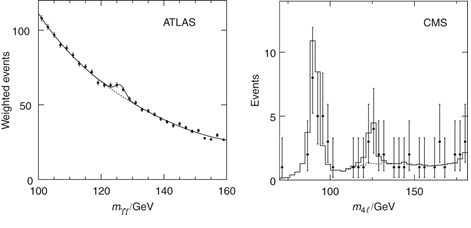
\includegraphics[width=0.75\textwidth,height=0.75\textheight,keepaspectratio]
                {pictures/higgs_results.png}
  \caption{Reconstructed invariant mass distribution plots. Solid lines
           indicate signal plus background expectation while dashed lines
           indicate background only expectation. The left corresponds to 
           $h\to\gamma\gamma$ decays measured at ATLAS while the right shows
           $h\to ZZ^{*}\to4\ell$ decays measured at CMS. Image taken from 
           Thomson Fig. 17.19 \cite{thomson_modern_2013}.}
  \label{fig:higgsevidence}
\end{figure}

\section{Future searches and conclusion}
There is still much about the
Higgs we must investigate and properties we must verify. We don't know, for
instance, if it is even under CP or whether it is spin-0. We 
haven't yet demonstrated that the Higgs couples to itself. The choice of one 
Higgs doublet is the most conservative, but it is possible to use more; in 
particular supersymmetric theories utilize at least two Higgs doublets 
\cite{thomson_modern_2013}. Finally, it is possible that the 
Higgs is a composite particle. 

\bibliographystyle{unsrtnat}
\bibliography{bibliography}
                               

